\chapter{Graphs}
\label{chp:graphs}
In this chapter are introduced the fundamentals concepts of \textbf{graphs} as mathematical objects, and as an abstract data type, its applications in computer science, and the most important and notable algorithms with their implementation. 
 
\section{General Definitions}
A graph is a discrete mathematical structure in which the connections between its elements, and their relationship are highlighted. A graph is made up by two different elements: \textbf{nodes} or \textbf{vertices}, and \textbf{links} or \textbf{edges}. In case the links do not have any direction the graph is called \textbf{undirected graph} (Figure), in case instead the links have a direction the graph is called \textbf{directed graph}.

\begin{figure}[H]
	\begin{center}
		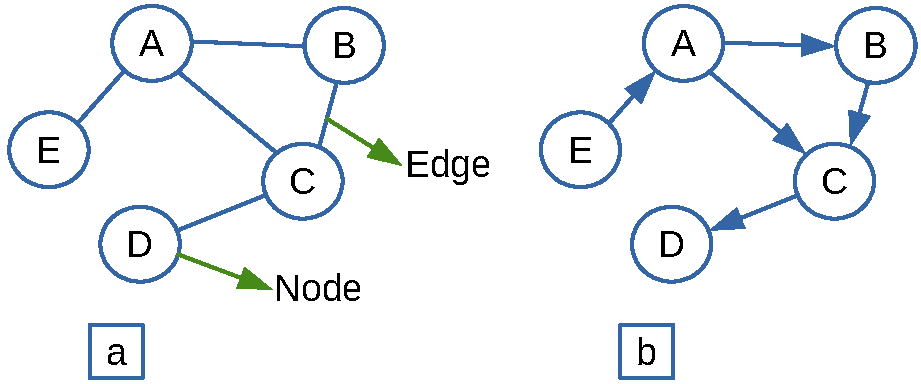
\includegraphics[scale=.6]{chapters/graphs/images/graphs_1.pdf}
		\caption[Undirected (a) and directed (b) graphs and its elements.]{Undirected (a) and directed (b) graphs and its elements.}
		\label{graphs_1}
	\end{center}
\end{figure}

Formally a graph is the pair \(G=(V, E)\), where \(V\) is the set of all vertices, and \(E\) is the set of paired vertices, whose elements are called edges \cite{wikigraphmath} (\href{https://en.wikipedia.org/wiki/Graph_(discrete_mathematics)}{Graph, Wikipedia}).

A \textbf{tree} (Chapter \ref{chp:trees}) is a special kind of graph.

Graphs are very useful to describe a lot of real situations like: connections between people, computers (internet), web pages (world wide web), airports, cities, and gene inside the DNA.

In graphs, differently to trees, closed loops can exist. These kind of closed loops can be dangerous for the algorithms because they could lead to infinite executions.

\subsection{Connectivity}
\textbf{Connectivity} is a measure that describe how much the nodes of a graph are connected. It is defined as the minimum number of elements (nodes or edges) that need to be removed to separate the remaining nodes into isolated subgraphs \cite{wikiconnectivity} (\href{https://en.wikipedia.org/wiki/Connectivity_(graph_theory)}{Connectivity, Wikipedia}).

A graph is said to be \textbf{connected} if every pairs of nodes are connected. Thus it always exists at least one path that connects every pairs of nodes. If an undirected graphs is not connected then it is \textbf{disconnected}: in this case there is one or more nodes that can not be reached by any paths.

\paragraph{Strongly Connected}
A directed graph is said to be \textbf{strongly connected} if every pairs of nodes can be reached by one or more path.

\paragraph{Weakly Connected}
A directed graph is said to be \textbf{weakly connected} if by replacing all the direct edges with undirectd ones, the new graph is connected. in a directed graph some nodes can not be reached if all the edges exit or enter from them. The graph in Figure \ref{graphs_2} is weakly connected because the node \(U\) has only entering edges.

\begin{figure}[H]
	\begin{center}
		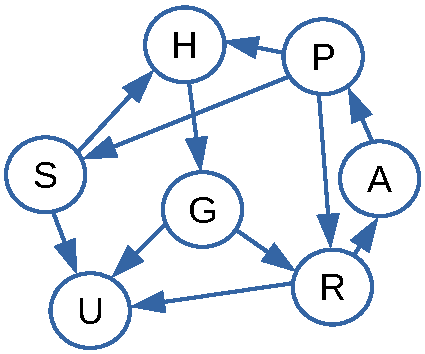
\includegraphics[scale=.6]{chapters/graphs/images/graphs_2.pdf}
		\caption[A weakly connected graph.]{A weakly connected graph.}
		\label{graphs_2}
	\end{center}
\end{figure}

\section{Graph Representations}
There are several ways to represent graphs using data structures. For example in an object oriented programming language a way could be to define a type for the vertex, and a type for the edges.

The most common data structures used for representing a graph are: \textbf{edge list}, \textbf{adjacency list}, and \textbf{adjacency matrix} \cite{goodrich2013data}. 

In appendix \ref{graphsappendix} there is a summary of the complexities for the most common operations performed on graphs for the different data structures.

\subsection{Edge List}
The \textbf{edge list} is an unordered list of all pairs of nodes that form an edge. This representation is minimal but it does not allow to locate a specific edge, or the set of edges incident to a particular node \cite{goodrich2013data}.

\begin{figure}[H]
	\begin{center}
		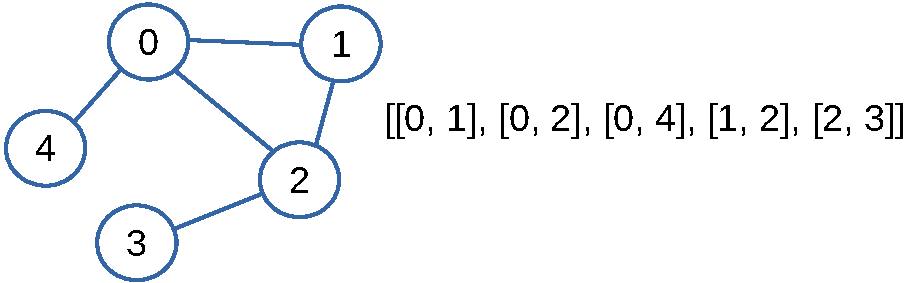
\includegraphics[scale=.6]{chapters/graphs/images/graphs_3.pdf}
		\caption[Edge list.]{Edge list.}
		\label{graphs_3}
	\end{center}
\end{figure}

\subsection{Adjacency List}
The \textbf{adjacency list} is a list containing a separate list for each node containing all the incident edges of that node. In this representation identify all the edges incident to a node is easy \cite{goodrich2013data}. In case of directed graphs for each node there are two different lists: one for entering edges, and another one for the edges that go out.

\begin{figure}[H]
	\begin{center}
		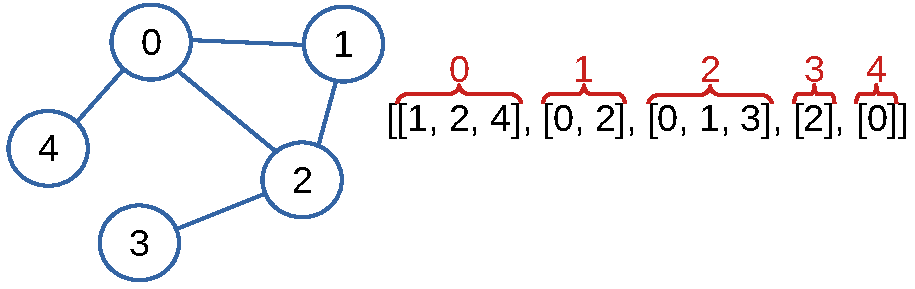
\includegraphics[scale=.6]{chapters/graphs/images/graphs_4.pdf}
		\caption[Adjacency list.]{Adjacency list.}
		\label{graphs_4}
	\end{center}
\end{figure}

\subsection{Adjacency Matrix}
The \textbf{adjacency matrix} is a matrix \(A\) in which each element \(A[i, j]\) represent the relationship between the edge \(i\) with the edge \(j\). If between \(i\) and \(j\) there is an edge \(A[i, j] = 1\), otherwise \(0\). In case the an ed go out and enter in the same edge \(A[i, i] = 1\). For undirected graphs this matrix is symmetric, and in case there are not edges going in and out the same node the principal diagonal is all of \(0\).

\begin{figure}[H]
	\begin{center}
		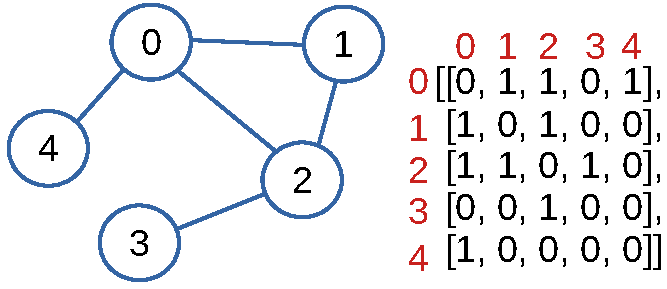
\includegraphics[scale=.6]{chapters/graphs/images/graphs_5.pdf}
		\caption[Adjacency matrix.]{Adjacency matrix.}
		\label{graphs_5}
	\end{center}
\end{figure}

In the appendix \ref{graphimplementationappendix} there is the full python implementation of the graph representation. There are defined the classes for nodes, edges, and graphs objects. Moreover, all the main operations on graphs like: insert a new node, a new edge, get the edge list, the adjacency list, the adjacency matrix, and find the max index are also implemented.

\section{Graph Traversal}
Like in the case of trees (Chapter \ref{chp:trees}), also for graphs there are two different ways of traverse: \textbf{depth-first search}, and \textbf{breadth-first search}. But for graphs, differently from trees, there is not a privileged way of traverse, and it is arbitrarily chosen a node where to start the traverse.

\subsection{Depth-first Search (DFS)}
In the \textbf{depth-fist search} the search starts from an arbitrary node and traverse one of the connected node. This process is repeated until there are not any new nodes on that path and start again with new nodes, until the searched node is found, or all the nodes have been traversed \cite{wikidepthfirst} (\href{https://en.wikipedia.org/wiki/Depth-first_search}{Depth-first search, Wikipedia}). This traversal can be implemented both recursively, and iteratively by using a stack.

\begin{figure}[H]
	\begin{center}
		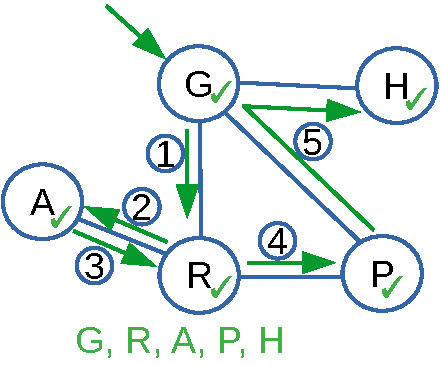
\includegraphics[scale=.6]{chapters/graphs/images/graphs_6.pdf}
		\caption[Depth-first search example.]{Depth-first search example.}
		\label{graphs_6}
	\end{center}
\end{figure}

\begin{lstlisting}[firstnumber=1, caption={Recursive implementation of a depth-first search.}]
class Graph():
	...
	
	def depth_first_search_recursive(self, start_node):
		ret_list = [start_node.value]
		start_node.visited = True
		edges_out = [e for e in start_node.edges
					 if e.node_to.value != start_node.value]
		for e in edges_out:
			if not edge.node_to.visited:
				ret_list.extend(depth_first_search_recursive(edge.node_to)
		return ret_list
\end{lstlisting}

The complexity in this case is \(O(\vert E \vert + \vert V \vert)\), where \(E\) is the number of edges and \(V\) the number of vertexes. For more details on complexities evaluation on graphs refer here \cite{goodrich2013data}.

In appendix \ref{graphimplementationtraversalappendix} there is a detailed recursive and iterative implementation, with also an additional example.
\subsection{Breadth-first Search (BFS)}
In \textbf{breadth-first search} the traversal is done starting from a node, and the firsy visited nodes are all its neighbors. Once visited all the neighbors the traversal keeps going in the same previous way \cite{wikibreadthfirst} (\href{https://en.wikipedia.org/wiki/Breadth-first_search}{Breadth-first search, Wikipedia}).

\begin{figure}[H]
	\begin{center}
		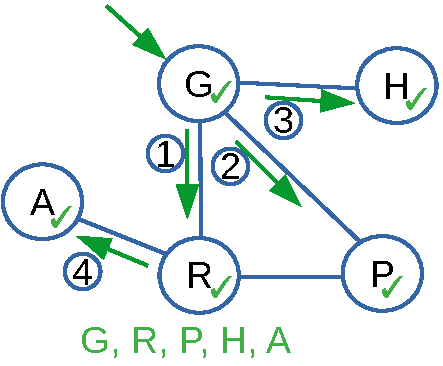
\includegraphics[scale=.6]{chapters/graphs/images/graphs_7.pdf}
		\caption[Breadth-first search example.]{Breadth-first search example.}
		\label{graphs_7}
	\end{center}
\end{figure}

The only possible implementation is the iterative one, and it is implemented by using a queue.

\begin{lstlisting}[firstnumber=1, caption={Recursive implementation of a depth-first search.}]
class Graph():
	...
	
	def breadth_first_search(self, start_node):
		
		return ret_list
\end{lstlisting}

The complexity in this case is \(O(\vert E \vert + \vert V \vert)\), where \(E\) is the number of edges and \(V\) the number of vertexes. For more details on complexities evaluation on graphs refer here \cite{goodrich2013data}.

In appendix \ref{graphimplementationtraversalappendix} there is the detailed implementation, with also an additional example.
\subsection{Eulerian Path and Circuit}
An \textbf{Eulerian path} (or \textbf{Eulerian trail}) is a path of edges that visits all the edges in a graph exactly once \cite{wikieulerianpathcircuit} (\href{https://en.wikipedia.org/wiki/Eulerian_path}{Eulerian path, Wikipedia}). Not every graph has an Eulerian path, and even if a graph has an Eulerian path it could be found only at specific starting nodes (Figure \ref{graphs_8}).

\begin{figure}[H]
	\begin{center}
		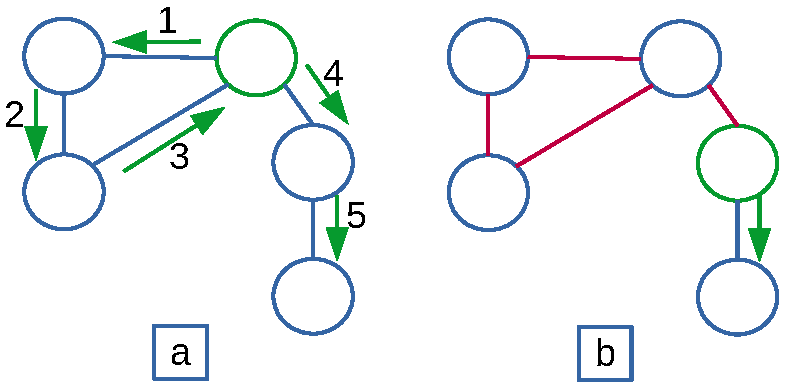
\includegraphics[scale=.6]{chapters/graphs/images/graphs_8.pdf}
		\caption[Eulerian path (a) and not Eulerian path (b).]{Eulerian path (a) and not Eulerian path (b).}
		\label{graphs_8}
	\end{center}
\end{figure}

An \textbf{Eulerian circuit} (or \textbf{Eulerian cycle}) is an Eulerian path which starts and ends on the same node. As before not every graph has an Eulerian circuit.

\begin{figure}[H]
	\begin{center}
		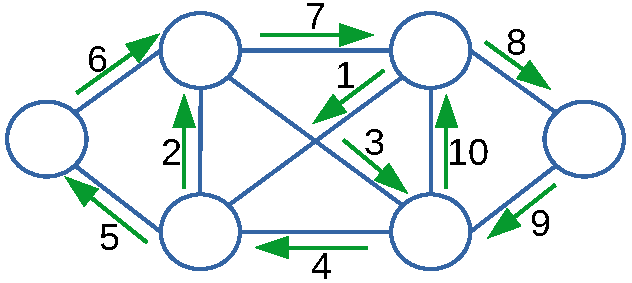
\includegraphics[scale=.6]{chapters/graphs/images/graphs_9.pdf}
		\caption[Eulerian circuit.]{Eulerian circuit.}
		\label{graphs_9}
	\end{center}
\end{figure}

In the following table are summarized some rules for finding if a graph has Eulerian path and/or circuit \cite{eulerpathcircuit}.

\begin{table}[H]
	\caption[Eulerian path and circuit existence rules.]{Eulerian path and circuit existence rules.}
	\label{eulerpathcircuit}
	\centering
	\begin{tabular}{| l | p{0.33\linewidth} | p{0.33\linewidth} |}
		\hline
 			& \textbf{Eulerian Path} & \textbf{Eulerian Circuit} \\
		\hline
		\textbf{Undirected Graph} & Either every vertex has even degree or exactly two vertices have odd degree. &  Every vertex has an even degree. \\
		\hline
		\textbf{Directed Graph} & At most one vertex has \newline (outdegree)-(indegree)=1 and at most one vertex has \newline (indegree)-(outdegree)=1 and all other vertices have equal in and out degrees. & Every vertex has equal indegree and outdegree. \\
		\hline
	\end{tabular}
\end{table}

\subsection{Hamiltonian Path and Circuit}
A \textbf{Hamiltonian path} (or \textbf{traceable path}) is a path in which all nodes are visited exactly once. A \textbf{Hamiltonian circuit} (or \textbf{Hamiltonian Cycle}) is a Hamiltonian path that starts and ends in the same node \cite{wikihamiltoninanpathcircuit} (\href{https://en.wikipedia.org/wiki/Hamiltonian_path}{Hamiltonian path, Wikipedia}).

\begin{figure}[H]
	\begin{center}
		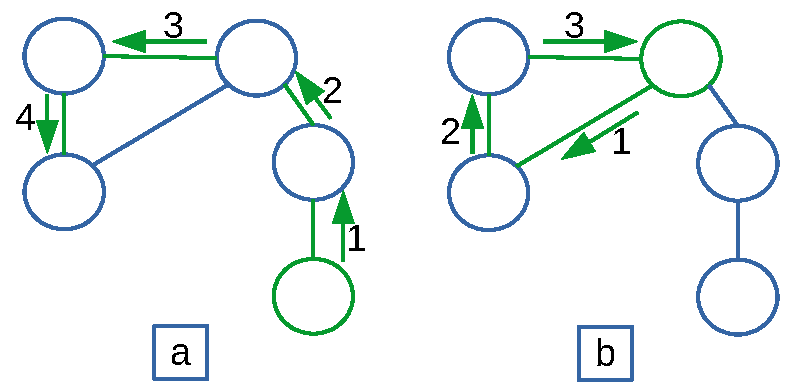
\includegraphics[scale=.6]{chapters/graphs/images/graphs_10.pdf}
		\caption[Hamiltonian path (a) and Hamiltonian circuit (b).]{Hamiltonian path (a) and Hamiltonian circuit (b).}
		\label{graphs_10}
	\end{center}
\end{figure}

\subsection{Shortest Path Problem}
The \textbf{shorted path problem} is the problem of finding a path between two nodes such that the sum of the weights is minimized. In case of an undirected graph the shortest path is the path that pass through the minimum number of nodes \cite{wikishortestpath} (\href{https://en.wikipedia.org/wiki/Shortest_path_problem}{Shortest path problem, Wikipedia}).The breadth-first search can be used for finding the shortest path from a node to all the others, but it expects that all the edges are of the same nature, and in several situation this approach is not useful. Let us image we would like to find the best path connecting two cities. In this case the links between the nodes are not the same, as some strees are faster or slower than others. Another interesting application of finding the shortest path in graphs is about routing packages from a computer to another in internet in order to be as fast as possible.

\begin{figure}[H]
	\begin{center}
		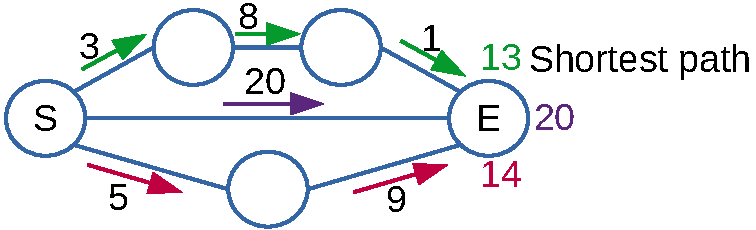
\includegraphics[scale=.6]{chapters/graphs/images/graphs_11.pdf}
		\caption[Shortest path.]{Shortest path.}
		\label{graphs_11}
	\end{center}
\end{figure}

\subsection{Dijkstra's Algorithm}
The Dijkstra's algorithm single source shortest path for a non-negative weighted graphs, in which all the shortest paths from a given node to all the other nodes are found. The distance between two nodes is the sum of the weights of the edges of the path.

This algorithm is part of a broader class of algorithms which is called \textbf{greedy algorithms} \cite{wikigreedy} (\href{https://en.wikipedia.org/wiki/Greedy_algorithm}{Greedy algorithms, Wikipedia}). In greedy algorithms the optimal solution is found by finding the optimal solution at every step without considering the previous ones. This approach does not always find the optimal solution of a problem. A more advanced technique to greedy algorithm is \textbf{dynamic programming}, which will be the topic of the next chapter.

\paragraph{Relaxation}
Before introducing the Dijkstra's algorithm it is important to introduce the \textbf{relaxation condition}. Let us consider the following weighted directed graph Figure \ref{graphs_12}. The cost for going from node 1 to node 2 is \(2\), and \(\infty\) from 1 to 3, as there is not any direct link. The relaxation condition is then:

\begin{definition}[Relaxation condition]
\enspace \enspace \textnormal{if (d[u] + w(u, v) < d[v])}

\enspace \enspace \enspace     \textnormal{d[v] = d[u] + w(u, v)}

Where \(d[u]\) is the distance of node u from the starting node (1 in this case), and \(w(u, v)\) is the weight from the node \(u\) to node \(v\).
\end{definition}

\begin{figure}[H]
	\begin{center}
		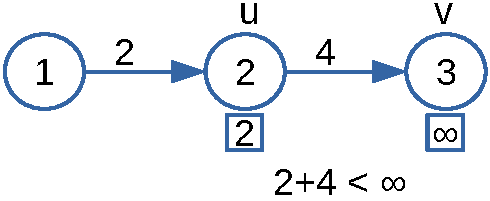
\includegraphics[scale=.6]{chapters/graphs/images/graphs_12.pdf}
		\caption[Relaxation condition.]{Relaxation condition.}
		\label{graphs_12}
	\end{center}
\end{figure}

In other words the relaxation condition says that if there is a shorter path connecting two nodes, this distance should be used as the new distance.

In the Dijkstra's algorithm at each step the new node is chosen based on the lowest value of the distance at that given step, and eventually the distances for all the adjacent nodes are updated accordingly the relaxation condition.

Let us consider the following graph Figure \ref{graphs_13}, and let us start from the node 1 \cite{dijkstraexplaination}.

\begin{figure}[H]
	\begin{center}
		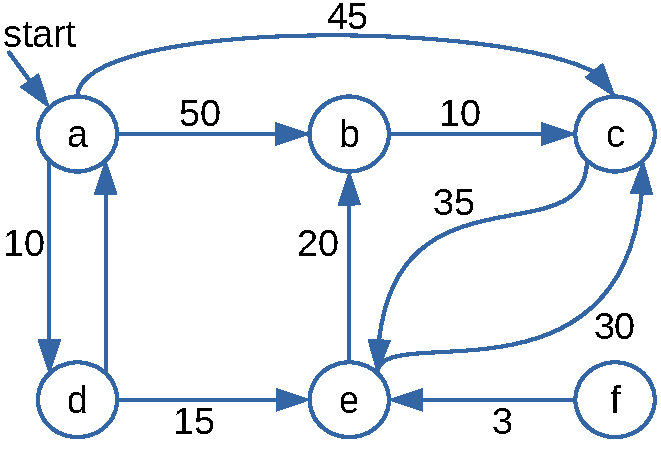
\includegraphics[scale=.6]{chapters/graphs/images/graphs_13.pdf}
		\caption[Dijkstra's algorithms example.]{Dijkstra's algorithm example.}
		\label{graphs_13}
	\end{center}
\end{figure}

For describing how the algorithm works we use the following table. At every step a new raw is added, and at the first one the table looks like the following:

\begin{table}[H]
\centering
\begin{tabular}{ l | c | c | c | c | c }
    selected vertex & 2 & 3 & 4 & 5 & 6 \\
    \hline
    4 & 50 & 45 & \mybox[rounded corners=6pt, line width=1pt, draw=red, fill=yellow!25]{mycol}{10} & \(\infty\) & \(\infty\)
\end{tabular}
\end{table}

All the nodes are listed as columns, and all the distances from the node 1 to all the others are reported in the table. The nodes 5 and 6 do not have any directed link to the node 1, then their distance is infinity. Once listed all the distances the node with the lowest one is selected: at the first step it is the node 4.

For second step all the distances of the adjacent nodes to 4 (in this case only for node 5) are updated except for the ones previously selected as the lowest. Once updated all the distances the process is repeated again, and the node with the lowest one is chosen (node 5 in this case).

\begin{table}[H]
\centering
\begin{tabular}{ l | c | c | c | c | c }
    selected vertex & 2 & 3 & 4 & 5 & 6 \\
    \hline
    4 & 50 & 45 & \mybox[rounded corners=6pt, line width=1pt, draw=black, fill=green!25]{mycol}{10} & \(\infty\) & \(\infty\) \\
    \hline
    5 & 50 & 45 & \mybox[rounded corners=6pt, line width=1pt, draw=black, fill=green!25]{mycol}{10} & \mybox[rounded corners=6pt, line width=1pt, draw=red, fill=yellow!25]{mycol}{25} & \(\infty\)
\end{tabular}
\end{table}

The process is repeated again: all the distances of the nodes adjacent to 5 are updated (in this case only the distance to node 2 (\(25+20\))).